\documentclass[letterpaper, 12pt]{article}

\usepackage{/Users/zhengz/Desktop/Math/Workspace/Homework1/homework}

%%%%%%%%%%%%%%%%%%%%%%%%%%%%%%%%%%%%%%%%%%%%%%%%%%%%%%%%%%%%%%%%%%%%%%%%%%%%%%%%%%%%%%%%%%%%%%%%%%%%%%%%%%%%%%%%%%%%%%%%%%%%%%%%%%%%%%%%
\begin{document}
%Header-Make sure you update this information!!!!
\noindent
%%%%%%%%%%%%%%%%%%%%%%%%%%%%%%%%%%%%%%%%%%%%%%%%%%%%%%%%%%%%%%%%%%%%%%%%%%%%%%%%%%%%%%%%%%%%%%%%%%%%%%%%%%%%%%%%%%%%%%%%%%%%%%%%%%%%%%%%
\large\textbf{Zhengdong Zhang} \hfill \textbf{Homework 1}   \\
Email: zhengz@uoregon.edu \hfill ID: 952091294 \\
\normalsize Course: MATH 682 - Algebraic Geometry II \hfill Term: Winter 2026 \\
Instructor: Professor Nick Addington \hfill Due Date: Jan 9th, 2026 \\
\noindent\rule{7in}{2.8pt}
\setstretch{1.1}
%%%%%%%%%%%%%%%%%%%%%%%%%%%%%%%%%%%%%%%%%%%%%%%%%%%%%%%%%%%%%%%%%%%%%%%%%%%%%%%%%%%%%%%%%%%%%%%%%%%%%%%%%%%%%%%%%%%%%%%%%%%%%%%%%%%%%%%%
% Exercise 1
%%%%%%%%%%%%%%%%%%%%%%%%%%%%%%%%%%%%%%%%%%%%%%%%%%%%%%%%%%%%%%%%%%%%%%%%%%%%%%%%%%%%%%%%%%%%%%%%%%%%%%%%%%%%%%%%%%%%%%%%%%%%%%%%%%%%%%%%
\begin{problem}{1}
\begin{enumerate}[(a)]
  \item Let \(R=\mathbb{Z}[\sqrt{-3}]\). Sketch the lattice in the complex plane. 
  \item Prove that \(R\) is not integrally closed using 
  \[\omega=e^{2\pi i/3}=\frac{-1+\sqrt{-3}}{2}.\]
  \item Prove that \(2\) is irreducible in \(R\) by reasoning with norms, where \(N(a+b\sqrt{-3})=a^2+3b^2\). But prove that \(2\) is not prime by showing that the quotient ring \(R/(2)\) is not an integral domain.
  \item Same for \(1+\sqrt{-3}\).
  \item Prove that the ideal \(\mathfrak{m}=(2,1+\sqrt{-3})\) is maximal by showing that the quotient ring \(R/\mathfrak{m}\) is a field. Prove that \(\mathfrak{m}\) is the only prime ideal containing \(2\) by reasoning about quotient rings. Same for \(1+\sqrt{-3}\).
  \item Prove that \(\mathfrak{m}^2=2 \mathfrak{m}\). Find the dimension of \(\mathfrak{m}/\mathfrak{m}^2\) as a vector space over \(R/\mathfrak{m}\). Prove that the principal ideal \((2)\) and \(1+\sqrt{-3}\) are not powers of \(\mathfrak{m}\), so they do not factor as products of primes. 
  \item Let \(S=\mathbb{Z}[\omega]\). Use the fact that \(S\) is a principal ideal domain to prove that the Krull dimension of \(R\) is 1.
  \item Let \(\mathfrak{n}=\mathfrak{m}S\). Prove that \(\mathfrak{n}\) is a principal ideal. Is it still prime? Describe the quotient ring \(S/\mathfrak{n}\) which should contain \(R/\mathfrak{m}\).
  \item Find the dimension of \(\mathfrak{n}/\mathfrak{n}^2\) as a vector space over \(S/\mathfrak{n}\).
\end{enumerate}
\end{problem}
\begin{solution}
\begin{enumerate}[(a)]
  \item The lattice is below:
  \[R=\left\{ a+b\sqrt{-3}\mid a,b\in \mathbb{Z} \right\}\]
  
  \begin{center}
  \begin{tikzpicture}[scale=0.8]
    % ==== Parameters ====
    \def\XMIN{-5} \def\XMAX{5}   % integer real parts
    \def\KMIN{-4} \def\KMAX{4}   % integer multipliers of sqrt(3) on the imaginary axis
    \def\SQRTTHREE{1.7320508075688772} % numeric value for sqrt(3)
  
    % Axes for the complex plane
    \draw[->, thick] (\XMIN,0) -- (\XMAX+0.3,0) node[below right] {$1$};
    \draw[->, thick] (0,\KMIN*\SQRTTHREE) -- (0,\KMAX*\SQRTTHREE+0.3) node[above left] {$\sqrt{-1}$};
  
    % Lattice points: z = x + k * sqrt(3) i, where x, k ∈ Z
    \foreach \x in {\XMIN,...,\XMAX}{
        \foreach \k in {\KMIN,...,\KMAX}{
            \pgfmathsetmacro{\y}{\k*\SQRTTHREE}
            \fill[blue!70] (\x,\y) circle[radius=1.2pt];
          }
      }
  
    % Optional labels for a few notable points
    \node[above right] at (0,0) {$\;0$};
    \node[above] at (0,\SQRTTHREE) {$\sqrt{-3}$};
    \node[below] at (1,\SQRTTHREE) {$1+\sqrt{-3}$};
  
    % Title
    %\node at (3.8,\KMAX*\SQRTTHREE-0.5) {\small Lattice $\{\,x + k\sqrt{3}\,i \mid x,k\in\mathbb{Z}\,\}$};
  \end{tikzpicture}
  \end{center}
  \item Since \(\omega=e^{2\pi i/3}\), it is easy to see that \(\omega^3-1=0\). So the minimal polynomial of \(\omega\) over \(R\) is \(x^2+x+1\). It is monic so \(\omega\) is integral over \(R\), but \(\omega\notin R\) as \(2\) is not invertible in \(R\). 
  \item Suppose \(2=\alpha\beta\) in \(R\) where \(\alpha,\beta\) are not units in \(R\). Then 
  \[4=N(2)=N(\alpha\beta)=N(\alpha)N(\beta).\]
  Since \(\alpha,\beta\) are not units, so \(N(\alpha)\neq 1\) and \(N(\beta)\neq 1\). This implies that 
  \[N(\alpha)=N(\beta)=2.\]
  It is easy to see that there exist no integers \(a,b\in \mathbb{Z}\) such that 
  \[a^2+3b^2=2.\]
  A contradiction. So \(2\) is irreducible in \(R\). 

  Now consider the quotient ring \(R/(2)\). \(1+\sqrt{-3}\) and \(1-\sqrt{-3}\) are nonzero elements in \(R/(2)\) because they are not multiples of \(2\). But 
  \[(1+\sqrt{-3})(1-\sqrt{-3})=4\equiv 0\]
  in \(R/(2)\). This implies \(R/(2)\) is not an integral domain. So \((2)\) is not a prime ideal in \(R\). 
  \item Note that \(N(1+\sqrt{-3})=N(2)=4\). The same argument as above implies that \(1+\sqrt{-3}\) is irreducible. For the quotient ring \(R/(1+\sqrt{-3})\). Note that  \(2\) is not a multiple of \(1+\sqrt{-3}\) in \(R\) and 
  \[2^2=(1+\sqrt{-3})(1-\sqrt{-3})\in (1+\sqrt{-3}).\]
  So \(2\) is a nilpotent element in \(R/(1+\sqrt{-3})\). This tells us that \(1+\sqrt{-3}\) is not prime.
  \item Consider the following map 
  \begin{align*}
       f:R&\rightarrow \mathbb{F}_2,\\
         1&\mapsto 1,\\
         \sqrt{-3}&\mapsto 1.
  \end{align*}
  It is a well-defined surjective ring map as in \(R\), we have \((\sqrt{-3})^2+3=0\) and in \(\mathbb{F}_2\), we have \(1^2+3=0\). It is easy to see that \(f(2)=f(1)+f(1)=0\) and \(f(1+\sqrt{-3})=f(1)+f(\sqrt{-3})=1+1=0\), so 
  \[\mathfrak{m}=(2,1+\sqrt{-3})\subset \ker f.\]
  Conversely, suppose \(a+b\sqrt{-3}\in R\) satisfies that 
  \[f(a+b\sqrt{-3})=af(1)+bf(\sqrt{-3})=a+b=0\]
  in \(\mathbb{F}_2\). So \(a+b\in \mathbb{Z}\) is even. Write 
  \[a+b\sqrt{-3}=a-b+b(1+\sqrt{-3}).\]
  Here \(a-b\) is also even as \(a+b\) is even. So \(a+b\sqrt{-3}\in (2,1+\sqrt{-3})\). This proves that 
  \[\ker f=(2,1+\sqrt{-3})=\mathfrak{m}.\]
  Hence, the quotient ring \(R/\mathfrak{m}\cong \mathbb{F}_2\) is a field and \(\mathfrak{m}\) is a maximal ideal. 

  Now suppose \(\mathfrak{p}\) is a prime ideal and \(2\in \mathfrak{p}\). We have 
  \[(1+\sqrt{-3})(1-\sqrt{-3})=2\cdot 2\in \mathfrak{p}.\]
  Because \(\mathfrak{p}\) is prime, so \(1+\sqrt{-3}\in \mathfrak{p}\). So we have 
  \[\mathfrak{m}=(2,1+\sqrt{-3})\subset \mathfrak{p}.\]
  We have proved that \(\mathfrak{m}\) is maximal, so \(\mathfrak{p}=\mathfrak{m}\). Similarly, if \(1+\sqrt{-3}\in \mathfrak{p}\), then by the same argument that \(2\in \mathfrak{p}\), so again \(\mathfrak{p}=\mathfrak{m}\).
  \item Write 
  \begin{align*}
       \mathfrak{m}^2&=(4,-2+2\sqrt{-3},2+2\sqrt{-3}),\\
       2\mathfrak{m}&=(4,2+2\sqrt{-3}).
  \end{align*}
  It is easy to see that 
  \[-2+2\sqrt{-3}=(2+2\sqrt{-3})-4.\]
  So \(\mathfrak{m}^2=2\mathfrak{m}\). We first prove a claim.
  \begin{claim}
    Any element in the ideal \(\mathfrak{m}=(2,1+\sqrt{-3})\) can be written as \(2a+b(1+\sqrt{-3})\) for \(a,b\in \mathbb{Z}\).
  \end{claim}
  \begin{claimproof}
    By definition, every element in \((2,1+\sqrt{-3})\) can be written as 
    \[2a+b(1+\sqrt{-3})\ \ \ \mathrm{where}\ \ a,b\in \mathbb{Z}[\sqrt{-3}].\]
    Suppose \(a=p+q\sqrt{-3}\) for \(p,q\in \mathbb{Z}\). We can rewrite 
    \[2(p+q\sqrt{-3})+b(1+\sqrt{-3})=2(p-q)+(b+2q)(1+\sqrt{-3}).\]
    So we can assume \(a\in \mathbb{Z}\). Now suppose \(b=m+n\sqrt{-3}\) for \(m,n\in \mathbb{Z}\), we can rewrite 
    \[2a+(m+n\sqrt{-3})(1+\sqrt{-3})=2(a-2n)+(m+n)(1+\sqrt{-3}).\]
    In this way, we can make both \(a,b\in \mathbb{Z}\).
  \end{claimproof}

  Now write an element in \(\mathfrak{m}\) as 
  \[2a+b(1+\sqrt{-3})\]
  for \(a,b\in \mathbb{Z}\). When view it as an element in \(\mathfrak{m}/\mathfrak{m}^2=\mathfrak{m}/2 \mathfrak{m}\), it has four possibilities depending on \(a\) is even or odd and \(b\) is even or odd. This means \(\mathfrak{m}/\mathfrak{m}^2\) as an \(R/\mathfrak{m}\)-vector space has 4 different elements, so its dimension is \(2\).

  By induction, for \(n\geq 1\), we have \(\mathfrak{m}^n=2^{n-1}\mathfrak{m}\). Suppose \((2)=\mathfrak{m}^n\), then \(2\in (2^n,2^{n-1}(1+\sqrt{-3}))\). So there exists \(a,b,c,d\in \mathbb{Z}\) such that 
  \[2=2^n(a+b\sqrt{-3})+2^{n-1}(c+d\sqrt{-3})(1+\sqrt{-3}).\]
  This implies that 
  \begin{align*}
       2^{n-1}(2a+c-3d)&=2,\\
       2^{n-1}(2b+c+d)&=0.
  \end{align*}
  When \(n=1\), we know that \((2)\neq \mathfrak{m}\), so \(n=2\). Then 
  \begin{align*}
       2a+c-3d&=1,\\
       2b+c+d&=0.
  \end{align*}
  Take their difference and we have 
  \[2a-2b-4d=1.\]
  A contradiction. So \((2)\) is not powers of \(\mathfrak{m}\). Similarly, if \(1+\sqrt{-3}\in \mathfrak{m}^n\), we get two equations:
  \begin{align*}
          2^{n-1}(2a+c-3d)&=1,\\
          2^{n-1}(2b+c+d)&=1.
  \end{align*}
  This is only possible when \(n=1\), but we know that \((1+\sqrt{-3})\neq (2,1+\sqrt{-3})\). So \((1+\sqrt{-3})\) is also not powers of \(\mathfrak{m}\).
  \item It is easy to see that \(R\) is a subring of \(S\). Note that \(S=R[\omega]\), and \(\omega\) is integral over \(R\) as the minimal polynomial of \(\omega\) over \(R\) is \(x^2+x+1\). So \(R\subset S\) is an integral extension. Thus, \(\dim R=\dim S=1\) as \(S\) is a principal ideal domain. 
  \item Note that 
  \[\mathfrak{n}=\mathfrak{m}S=(2,1+\sqrt{-3})=(2,-1+\sqrt{-3})=(2,2\omega)=(2).\]
  So \(\mathfrak{n}\) is a principal ideal in \(S\). Consider the quotient ring \(S/\mathfrak{n}=\mathbb{Z}[\omega]/(2)=\mathbb{F}_2[\omega]\). This is the field adjoining a root of the polynomial \(x^2+x+1\). So \(S/(2)\cong \mathbb{F}_4\) is the splitting field of \(x^2+x+1\), which is the finite field with 4 elements. This implies \(\mathfrak{n}\) is a prime ideal. 
  \item The field \(S/\mathfrak{n}\) has 4 elements \(0,1,\omega,\omega^2=1+\omega\). The vector space \(\mathfrak{n}/\mathfrak{n}^2\) has only one generator \(2\), so its dimension over \(S/\mathfrak{n}\) is \(1\).
\end{enumerate}
\end{solution}

\noindent\rule{7in}{2.8pt}  
%%%%%%%%%%%%%%%%%%%%%%%%%%%%%%%%%%%%%%%%%%%%%%%%%%%%%%%%%%%%%%%%%%%%%%%%%%%%%%%%%%%%%%%%%%%%%%%%%%%%%%%%%%%%%%%%%%%%%%%%%%%%%%%%%%%%%%%%
% Exercise 2
%%%%%%%%%%%%%%%%%%%%%%%%%%%%%%%%%%%%%%%%%%%%%%%%%%%%%%%%%%%%%%%%%%%%%%%%%%%%%%%%%%%%%%%%%%%%%%%%%%%%%%%%%%%%%%%%%%%%%%%%%%%%%%%%%%%%%%%%
\begin{problem}{2}
\begin{enumerate}[(a)]
  \item Let \(R=\mathbb{R}[x,y]/(y^2+x^2-x^3)\). Sketch the curve in \(\mathbb{R}^2\).
  \item Prove that \(R\) is not integrally closed.
  \item Prove that \(x\) is irreducible in \(R\) by reasoning about degrees. But prove that \(x\) is not prime by showing that the quotient ring \(R/(x)\) is not an integral.
  \item Same for \(y\).
  \item Prove that the ideal \(\mathfrak{m}=(x,y)\) is maximal by showing that the quotient ring \(R/\mathfrak{m}\) is a field. Prove that \(\mathfrak{m}\) is the only prime ideal containing \(x\) by reasoning about quotient rings.
  \item Find the dimension of \(\mathfrak{m}/\mathfrak{m}^2\) as a vector space over \(R/\mathfrak{m}\). Prove that the principal ideal \((x)\) is not a power of \(\mathfrak{m}\), so it does not factor as a product of primes. 
  \item Let \(S=\mathbb{R}[z]\). Describe the normalization map \(\varphi:R\rightarrow S\) that sends \(y/x\) to \(z\): where does it send \(x\) and \(y\)? Prove that the Krull dimension of \(R\) is 1.
  \item Let \(\mathfrak{n}=\varphi(\mathfrak{m})S\). Prove that \(\mathfrak{n}\) is a principal ideal. Is it still prime? Describe the quotient ring \(S/\mathfrak{n}\), which should contain \(R/\mathfrak{m}\).
  \item Find the dimension of \(\mathfrak{n}/\mathfrak{n}^2\) as a vector space over \(S/\mathfrak{n}\).
\end{enumerate}
\end{problem}
\begin{solution}
\begin{enumerate}[(a)]
  \item The curve \(y^2+x^2-x^3=0\) is sketched below:
  
  \begin{center}
    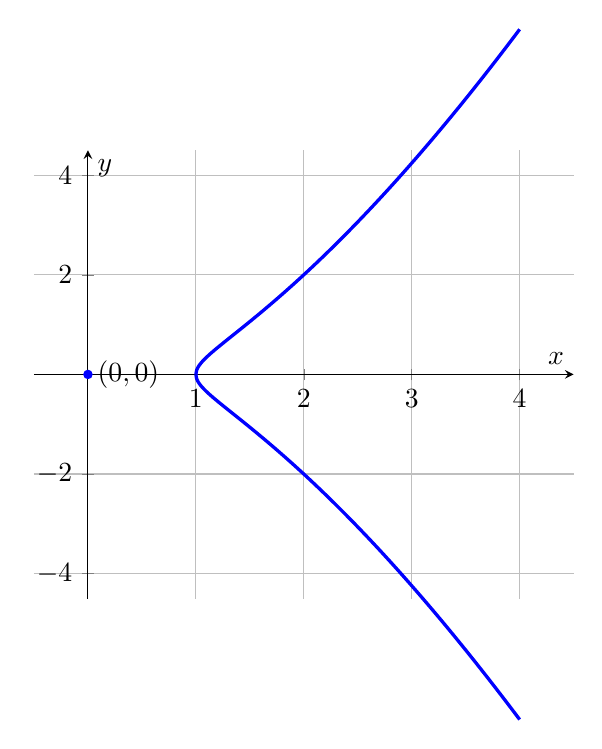
\begin{tikzpicture}
      \begin{axis}[
          axis lines=middle,
          xlabel={$x$}, ylabel={$y$},
          xmin=-0.5, xmax=4.5,
          ymin=-4.5, ymax=4.5,
          samples=400,
          clip=false,
          grid=both
        ]
        % Positive branch: y = x*sqrt(x-1), x >= 1
        \addplot[
          domain=1:4, smooth, very thick, blue
        ] {x*sqrt(x-1)};
    
        % Negative branch: y = -x*sqrt(x-1), x >= 1
        \addplot[
          domain=1:4, smooth, very thick, blue
        ] {-x*sqrt(x-1)};
    
        % Mark (1,0) and (0,0)
        \addplot[only marks, mark=*, mark size=1.5pt, blue] coordinates {(0,0)};
        %\node[anchor=west] at (axis cs:1,0) {$(1,0)$};
        \node[anchor=west] at (axis cs:0,0) {$(0,0)$};
      \end{axis}
    \end{tikzpicture}
  \end{center}
  \item Let \(z=y/x\) be an element in the fraction field of \(R\). And we have 
  \[z^2=\frac{y^2}{x^2}=\frac{x^3-x^2}{x^2}=x-1\in R.\]
  Next, we need to show that \(z\notin R\). Consider a monomial \(x^my^n\in \mathbb{R}[x,y]\). If \(n\geq 2\), we can replace \(y^2\) with \(x^3-x^2\) such that 
  \[x^my^n=x^m(x^3-x^2)y^{n-2}\]
  in \(R\). By doing so repeatedly, we can write every element in \(R\) in the form of \(f(x)+g(x)y\). Suppose there exists \(f,g\in \mathbb{R}[x]\) such that 
  \[\frac{y}{x}=f(x)+g(x)y.\]
  Then 
  \[y=xf(x)+xg(x)y.\]
  This means \(xg(x)=1\) for some \(g(x)\in \mathbb{R}[x]\). A contradiction. So \(z\notin R\). We have found an element \(z\) which is not in \(R\) but integral over \(R\), so \(R\) is not integrally closed. 
  \item Suppose \(x\) is not irreducible in \(R\). Then there exists \(f,g,h,k\in \mathbb{R}[x]\) such that 
  \[x=(f(x)+g(x)y)(h(x)+k(x)y).\]
  Expand and replace \(y^2\) with \(x^3-x^2\), we get 
  \[x=f(x)h(x)+(x^3-x^2)g(x)k(x)+[f(x)k(x)+g(x)h(x)]y.\]
  Let 
  \[\deg f=a,\ \ \deg g=b,\ \ \deg h=c,\ \ \deg k=d.\]
  From the equation, we get 
  \begin{align*}
       a+c&=b+d+3,\\
       a+d&=b+c.
  \end{align*}
  Take their difference and we get 
  \[2c-2d=3\]
  A contradiction. So \(x\) is irreducible in \(R\). Consider the quotient ring 
  \[R/(x)=\mathbb{R}[y]/(y^2).\]
  It is not an integral domain as \(y\) is a nilpotent element. So \(x\) is not prime.
  \item We use a similar argument to show that \(y\) is irreducible. In this case, we get 
  \[y=f(x)h(x)+(x^3-x^2)g(x)k(x)+[f(x)k(x)+g(x)h(x)]y.\]
  So 
  \begin{align*}
       a+c&=b+d+3,\\
       a+d&=b+c.
  \end{align*}
  Same argument implies that \(y\) is irreducible. Consider the quotient ring 
  \[R/(y)=\mathbb{R}[x]/(x^2-x^3).\]
  This is not an integral domain as \(x\) is a zero divisor. So \(y\) is not prime.
  \item It is not hard to see that 
  \[R/\mathfrak{m}=R/(x,y)\cong \mathbb{R}.\]
  So \(R/\mathfrak{m}\) is a field and \(\mathfrak{m}\) is maximal. Let \(\mathfrak{p}\) be a prime ideal and \(x\in \mathfrak{p}\). We know that \(R/\mathfrak{p}\) is an integral domain and \(y\in R/(x)\) is nilpotent. Note that 
  \[R/\mathfrak{p}\subset R/(x)=R[y]/(y^2).\]
  So \(R/\mathfrak{p}\) is a subring of \(R[y]/(y^2)\) and \(R/\mathfrak{p}\) does not contain \(y\). So \(R/\mathfrak{p}\cong \mathbb{R}\) and \(\mathfrak{p}\supset (x,y)=\mathfrak{m}\). We have proved \(\mathfrak{m}\) is maximal, so \(\mathfrak{p}=\mathfrak{m}\).
  \item Here \(\mathfrak{m}=(x,y)\) and \(\mathfrak{m}^2=(x^2,xy,y^2)\), so \(\mathfrak{m}/\mathfrak{m}^2\) only contains degree 1 polynomials and we have 
  \[\mathfrak{m}/\mathfrak{m}^2\cong \mathbb{R}x\oplus \mathbb{R}y.\]
  This implies that \(\mathfrak{m}/\mathfrak{m}^2\) is a 2-dimensional vector space over \(R/\mathfrak{m}\cong \mathbb{R}\).
  
  For \(n\geq 1\), the ideal \(\mathfrak{m}^n\) is generated by all monomials \(x^py^{n-p}\) for \(0\leq p\leq n\). For \(n-p\geq 2\), we can replace \(y^2\) with \(x^3-x^2\). Note that this does not decrease the degree of the monomial, so if \(x\in \mathfrak{m}^n\), \(n\) has to be 1. But we know \((x)\neq (x,y)=\mathfrak{m}\), so \((x)\) is not a power of \(\mathfrak{m}\), thus it does not factor as a product of primes.
  \item Consider the following map:
  \begin{align*}
       f: \mathbb{R}[x,y]&\rightarrow S=\mathbb{R}[z],\\
                x&\mapsto z^2+1,\\
                y&\mapsto z(z^2+1).
  \end{align*}
  It is easy to see that 
  \begin{align*}
       &f(y)^2+f(x)^2-f(x)^3\\
      =&z^2(z^2+1)^2+(z^2+1)^2-(z^2+1)^3\\
      =&(z^2+1)^2(z^2+1-z^2-1)\\
      =&0.       
  \end{align*}
  So \(y^2+x^2-x^3\in \ker f\) and the ideal \((y^2+x^2-x^3)\subset \ker f\). We know that the Krull dimenison of \(S\) is \(1\), and the image of \(f\) is a subring of \(S\). This implies that \(\ker f\) is a prime ideal of \(\mathbb{R}[x,y]\) and the Krull dimension of the quotient ring \(\mathbb{R}[x,y]/\ker f\) is also 1 as the image is not the field \(\mathbb{R}\). By 
  \[\mathrm{ht}\ker f+\dim \mathbb{R}[x,y]/\ker f=\mathrm{ht}\ker f+1\leq \dim \mathbb{R}[x,y]=2,\]
  We know that the height of the prime ideal \(\ker f\) is smaller or equal to \(1\). The ideal \((y^2+x^2-x^3)\) is a prime ideal contained in \(\ker f\) since \(y^2+x^2-x^3\) is irreducible, so \(\ker f=(y^2+x^2-x^3)\). The map \(f\) induces a well-defined map 
  \begin{align*}
       \varphi: &\mathbb{R}[x,y]/(y^2+x^2-x^3)=R\rightarrow S,\\
       x&\mapsto z^2+1,\\
       y&\mapsto z(z^2+1).
  \end{align*}
  By construction, the map \(\varphi\) sends \(y/x\) to \(z\) and is injective. So \(S\) is an integral extension of \(R\) and \(\dim R=\dim S=1\). 
  \item \(\mathfrak{n}=(z^2+1,z(z^2+1))=(z^2+1)\). This implies that \(\mathfrak{n}\) is a principal ideal generated by \(z^2+1\). Consider the quotient ring \(S/\mathfrak{n}=\mathbb{R}[z]/(z^2+1)\cong \mathbb{C}\). It is a field, so the ideal \(\mathfrak{n}\) is a maximal ideal, thus \(\mathfrak{n}\) is prime.
  \item For any \(f\in \mathbb{R}[z]\), use Euclidean algorithm, we can write 
  \[f(z)=g(z)(z^2+1)+r(z)\] 
  where \(r(z)=az+b\) for some \(a,b\in \mathbb{R}\). We know every element in \(\mathfrak{n}\) can be written as 
  \[f(z)(z^2+1)=g(z)(z^2+1)^2+(a+bz)(z^2+1).\]
  Here \(a+bz\) can be viewed as elements in \(S/\mathfrak{n}=\mathbb{R}[z]/(z^2+1)\). The vector space \(\mathfrak{n}/\mathfrak{n}^2\) is generated by one base \(z^2+1\), so the dimension is \(1\).
\end{enumerate}
\end{solution}

\noindent\rule{7in}{2.8pt}
%%%%%%%%%%%%%%%%%%%%%%%%%%%%%%%%%%%%%%%%%%%%%%%%%%%%%%%%%%%%%%%%%%%%%%%%%%%%%%%%%%%%%%%%%%%%%%%%%%%%%%%%%%%%%%%%%%%%%%%%%%%%%%%%%%%%%%%%
% Exercise 3
%%%%%%%%%%%%%%%%%%%%%%%%%%%%%%%%%%%%%%%%%%%%%%%%%%%%%%%%%%%%%%%%%%%%%%%%%%%%%%%%%%%%%%%%%%%%%%%%%%%%%%%%%%%%%%%%%%%%%%%%%%%%%%%%%%%%%%%%
\begin{problem}{3}
Find a square-free integer \(D\) with \(D\equiv 1\) (mod \(4\)) such that the maximal ideal \(\mathfrak{m}=(2,1+\sqrt{D})\) in \(R=\mathbb{Z}[\sqrt{D}]\) splits when you extend to \(S=\mathbb{Z}[\frac{1+\sqrt{D}}{2}]\)?
\end{problem}
\begin{solution}
Let \(D=-7\). We have \(-7\equiv 1\) (mod \(4\)). Let \(f:R\rightarrow S\) be the extension map and 
\[\mathfrak{n}=f(\mathfrak{m})S=(2,1+\sqrt{-7})=(2,2\cdot \frac{1+\sqrt{-7}}{2})=(2).\]
Note that \(2\) is not irreducible in \(S\) as 
\[\frac{1+\sqrt{-7}}{2}\cdot \frac{1-\sqrt{-7}}{2}=2.\]
So the ideal \(\mathfrak{n}\) splits into \((\frac{1+\sqrt{-7}}{2})\) and \((\frac{1-\sqrt{-7}}{2})\). 
\end{solution}



\end{document}